\documentclass{report}
\usepackage{titling} % For subtitle
\usepackage{tocloft} % For customizing TOC formatting
\usepackage{soul} % For highlighting text
\usepackage{xcolor}
\usepackage{graphicx}
\usepackage{tabularx} % for automatic column width adjustment


% Manually setting the margins
\setlength{\textwidth}{\dimexpr 15.4cm}  % Width of text area
\setlength{\textheight}{\dimexpr 23.4cm} % Height of text area
\setlength{\oddsidemargin}{-0.25in}      % Left margin (negative value reduces margin)
\setlength{\evensidemargin}{-0.25in}     % Even page left margin (for two-sided printing)
\setlength{\topmargin}{-0.5in}           % Top margin
\setlength{\headheight}{14pt}            % Space for header (optional)
\setlength{\headsep}{25pt}               % Space between header and text
\setlength{\footskip}{30pt}              % Distance from bottom of text to footer

% Set the main font to Helvetica
\usepackage[scaled]{helvet}
\renewcommand{\rmdefault}{phv}

% Set highlight colour
\sethlcolor{yellow}

\begin{document}

% Title Page Formatting

\includegraphics[width=0.5\textwidth]{Figures/tud_logo.png}
\title{MSc in Computing - Team Project}
%\title{User Evaluation Report - Magpie (Group 3)}
\author{Anais Blenet\\Saul Burgess\\Yuanshuo Du\\Jessica Fornetti\\Andreas Kraus\\Kaustubh Trivedi}
\date{\today}

% Customizing TOC formatting
\renewcommand{\cfttoctitlefont}{\hfill\Huge\bfseries} % Center TOC title
\renewcommand{\cftaftertoctitle}{\hfill}

\maketitle % Generates the title page

% Table of Contents
\tableofcontents
\newpage

% Main Body
\chapter{Introduction}
\section{Proposed Hypothesis}
Our project's goal is to provide a easy-to-use Geographical Information Service
in Dublin City. In our preliminary research, we couldn’t find a singular
system that allowed users to gain a general overview of public amenities, for
example, parking, bike infrastructure, or public transport. In Ireland and the
United Kingdom, the prevalence of proper digitised records in county
administrations varies wildly (Lynn et al., 2023). Some make use of
state-of-the-art geographical information systems (GIS) while others rely on
spreadsheets which are manually kept up to date. (McGuirk and MacLaran, 2001) A
system that would allow users to quickly inspect a combined dataset grounded in
automatically generated, real-world data could accelerate processes like planning permissions, urban development, or resource allocation.
Prior to user evaluation, exploratory work was conducted in the forms of a
market research survey to answer key demographic \& product questions:
\begin{enumerate}
    \item Who is our primary target user?
    \item What kind of amenity data do they access and how?
    \item What devices/tools do they primarily use?
    \item Are they satisfied with those tools?
    \item Would they consider Magpie useful in filling the gaps in their
          toolset?
\end{enumerate}
Responses from the survey further allowed us to confirm our target demographic
(figure 1.1), find out the proportion of users using amenity data for their work
(figure 1.2), what type of amenity data  they require access to (figure 1.3) and
why current tools are unsatisfactory (figure 1.4).
\begin{figure}
    \centering
    \begin{minipage}{0.45\textwidth}
        \centering
        \fbox{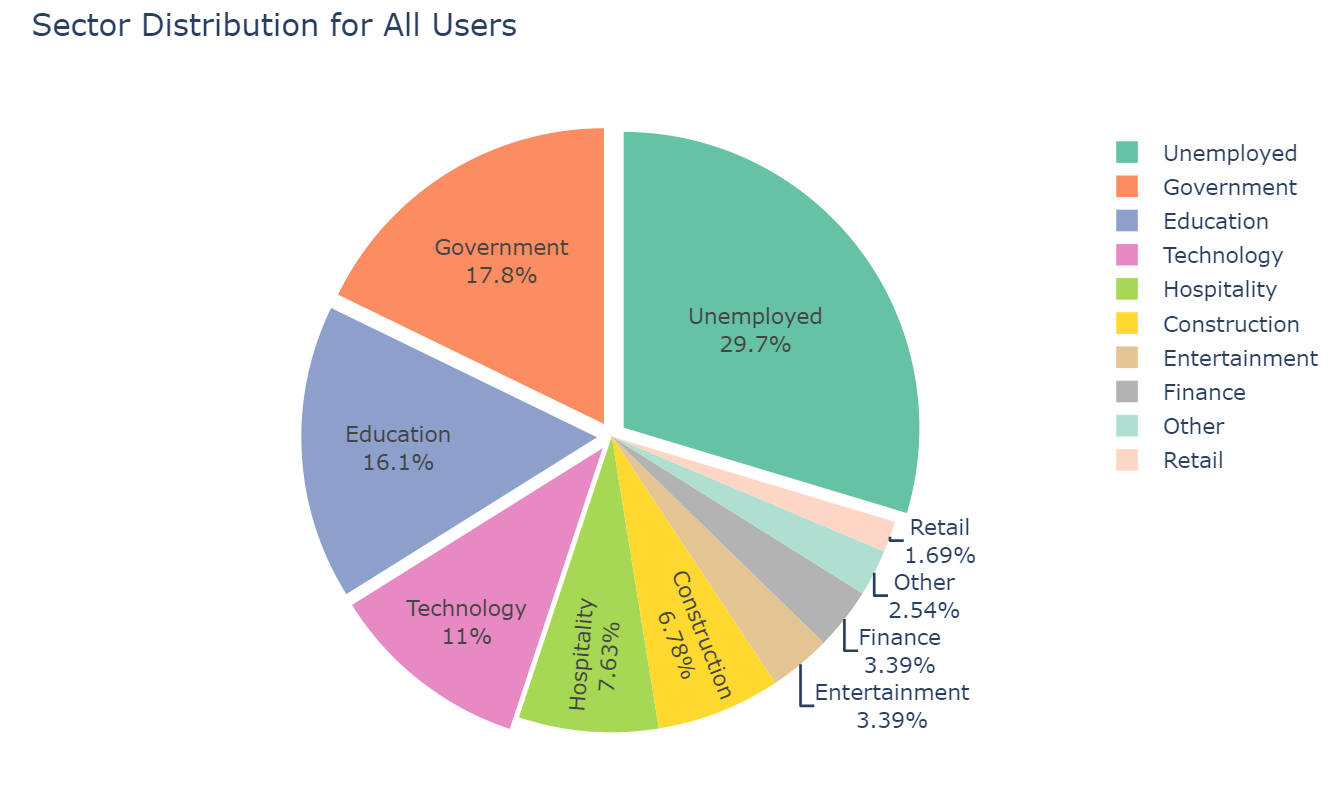
\includegraphics[width=\textwidth]{Figures/fig1.png}}
        \caption{Target user sectors}
        \label{fig:plot1}
    \end{minipage}
    \hfill
    \begin{minipage}{0.45\textwidth}
        \centering
        \fbox{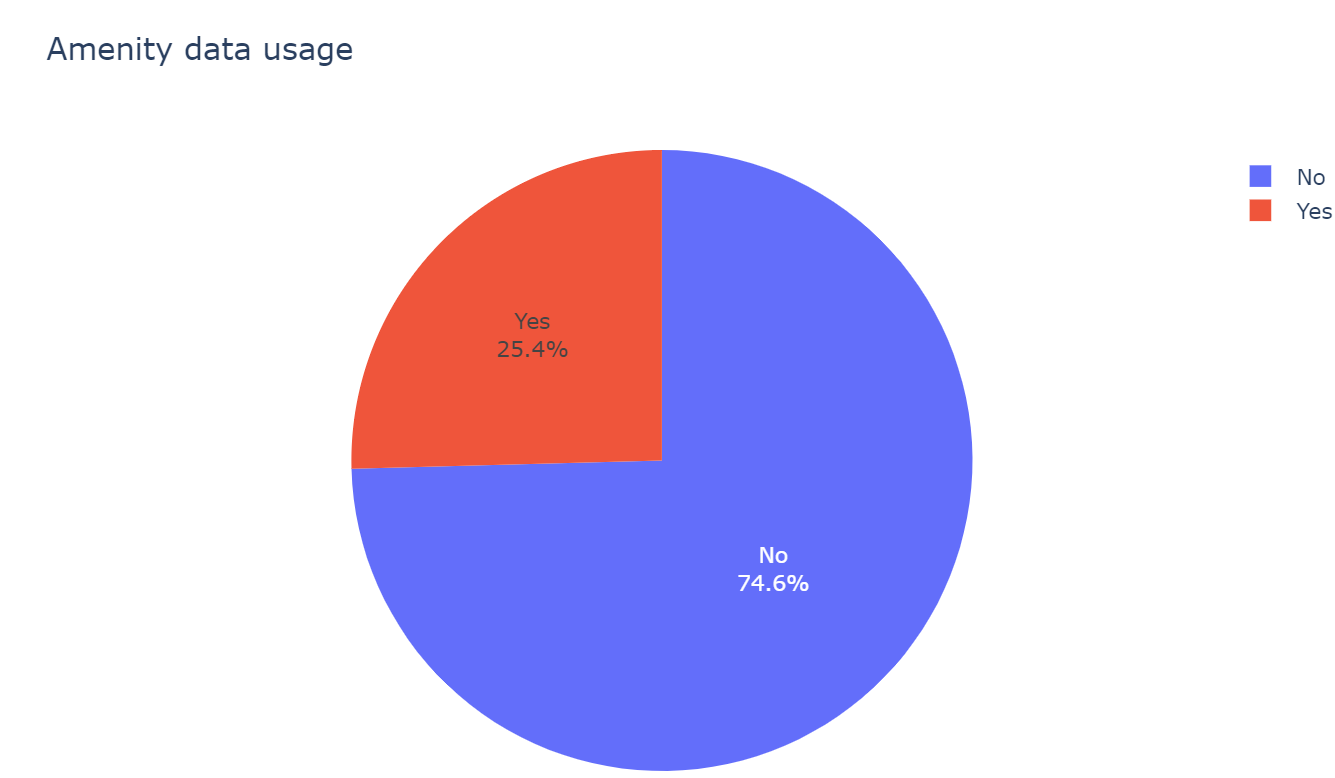
\includegraphics[width=\textwidth]{Figures/fig2.png}}
        \caption{Amenity Access distribution}
        \label{fig:plot2}
    \end{minipage}
\end{figure}
These responses also cemented the need of Magpie (figure 1.5) for both casual
users (User A) \& professionals who require amenity data (User B).
\begin{figure}
    \centering
    \begin{minipage}{0.5\textwidth}
        \centering
        \fbox{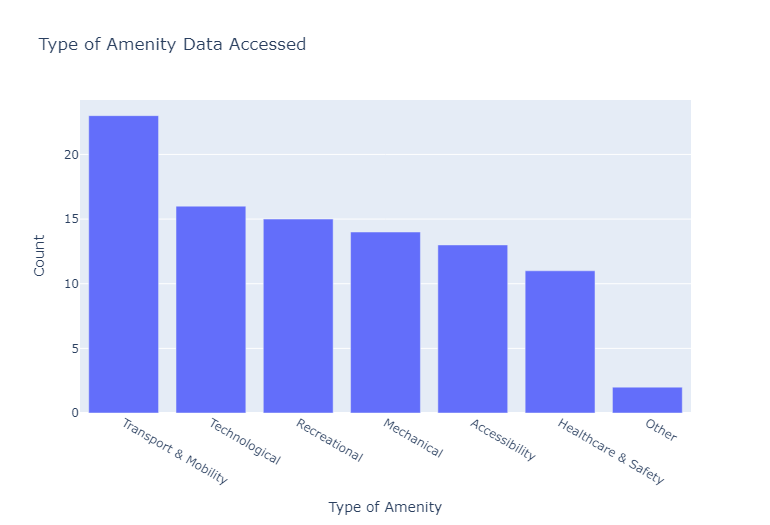
\includegraphics[width=\textwidth]{Figures/fig3.png}}
        \caption{Current amenity data accessed}
        \label{fig:plot3}
    \end{minipage}
    \hfill
    \begin{minipage}{0.6\textwidth}
        \centering
        \fbox{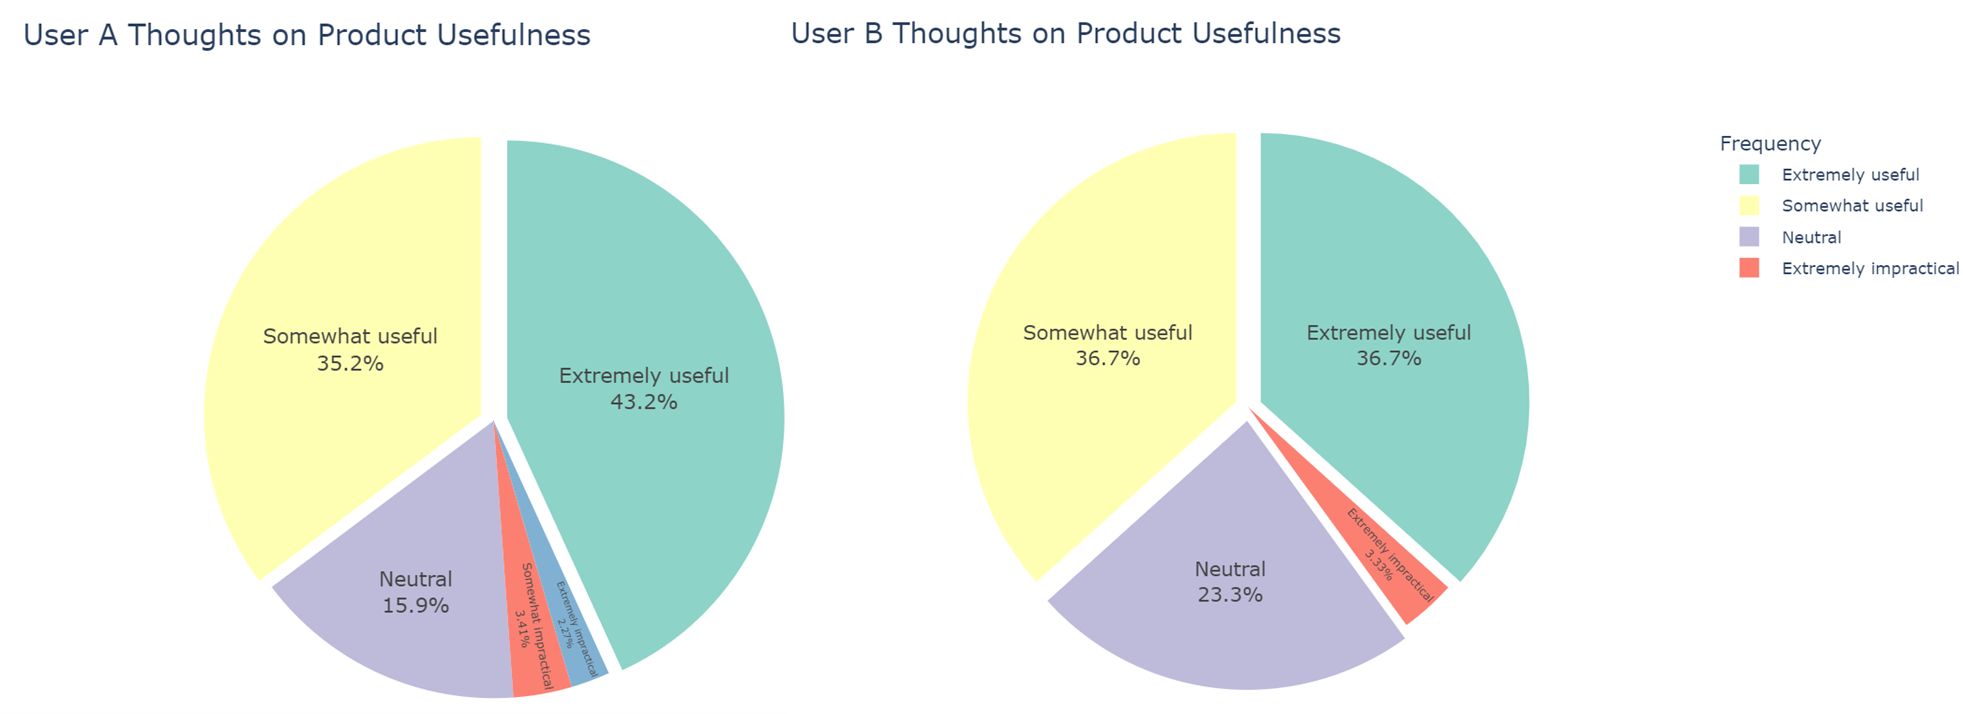
\includegraphics[width=\textwidth]{Figures/fig4.png}}
        \caption{Current tools \& satisfaction rate}
        \label{fig:plot4}
    \end{minipage}
    \hfill
    \begin{minipage}{0.6\textwidth}
        \centering
        \fbox{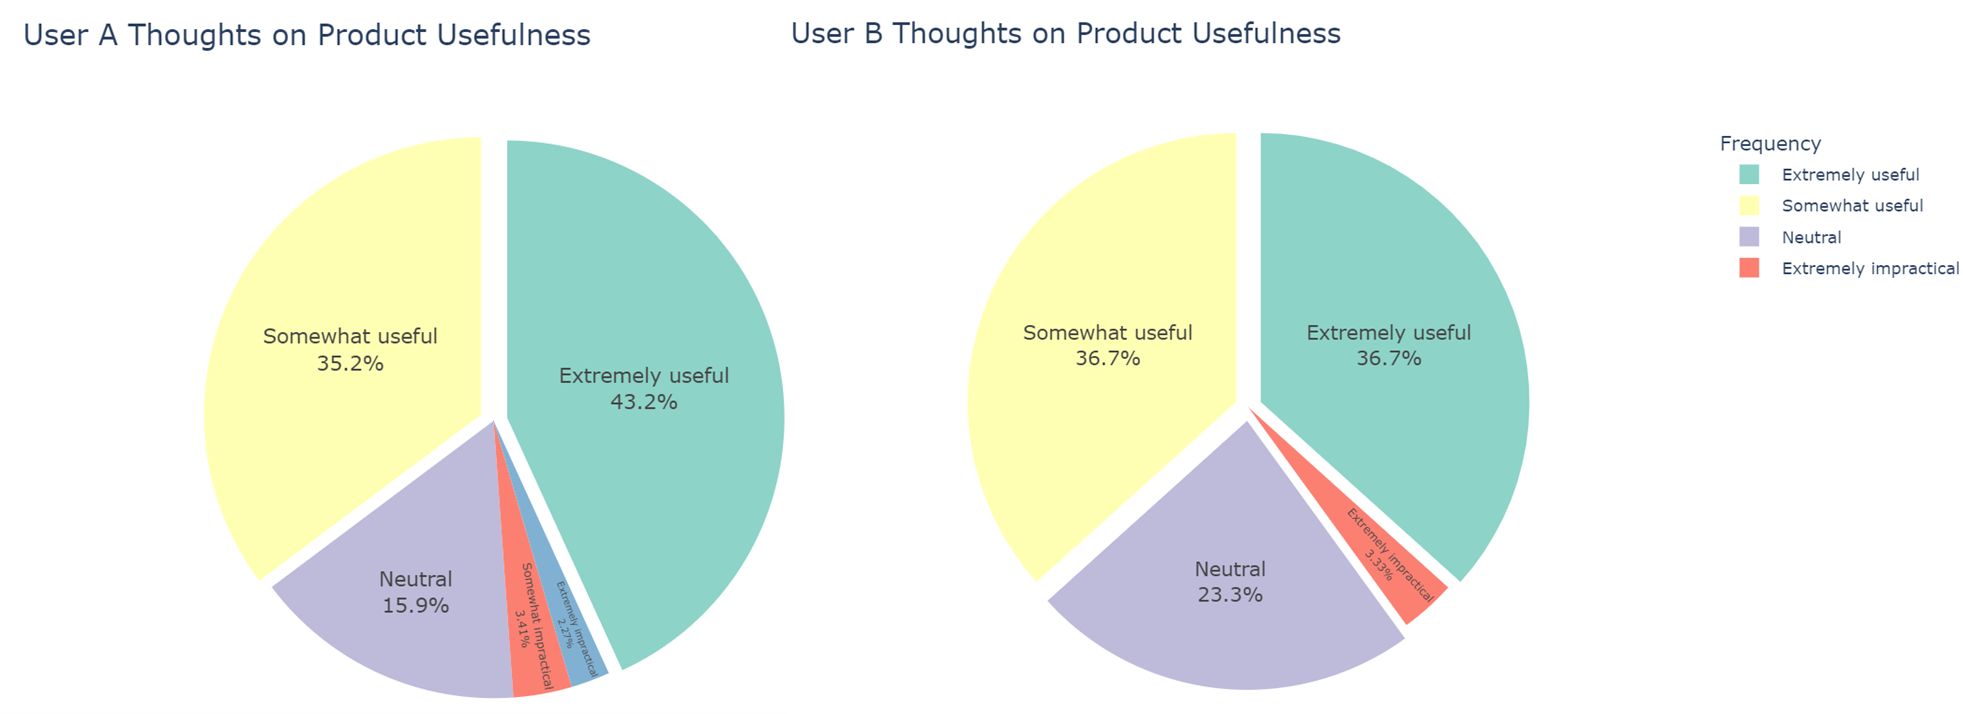
\includegraphics[width=\textwidth]{Figures/fig5.png}}
        \caption{Magpie potential}
        \label{fig:plot5}
    \end{minipage}
\end{figure}

\noindent{}The survey also helped us implement additional features (figure
1.6,1.7 \& 1.8) prior to the user evaluation such as a dashboard with search functionality and filters.\\ \\

\begin{figure}
    \centering
    \begin{minipage}{0.45\textwidth}
        \centering
        \fbox{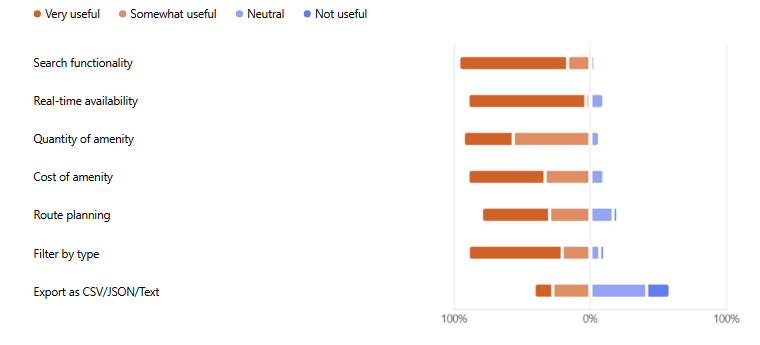
\includegraphics[width=\textwidth]{Figures/fig6.png}}
        \caption{Additional features rating}
        \label{fig:plot6}
    \end{minipage}
    \hfill
    \begin{minipage}{0.45\textwidth}
        \centering
        \fbox{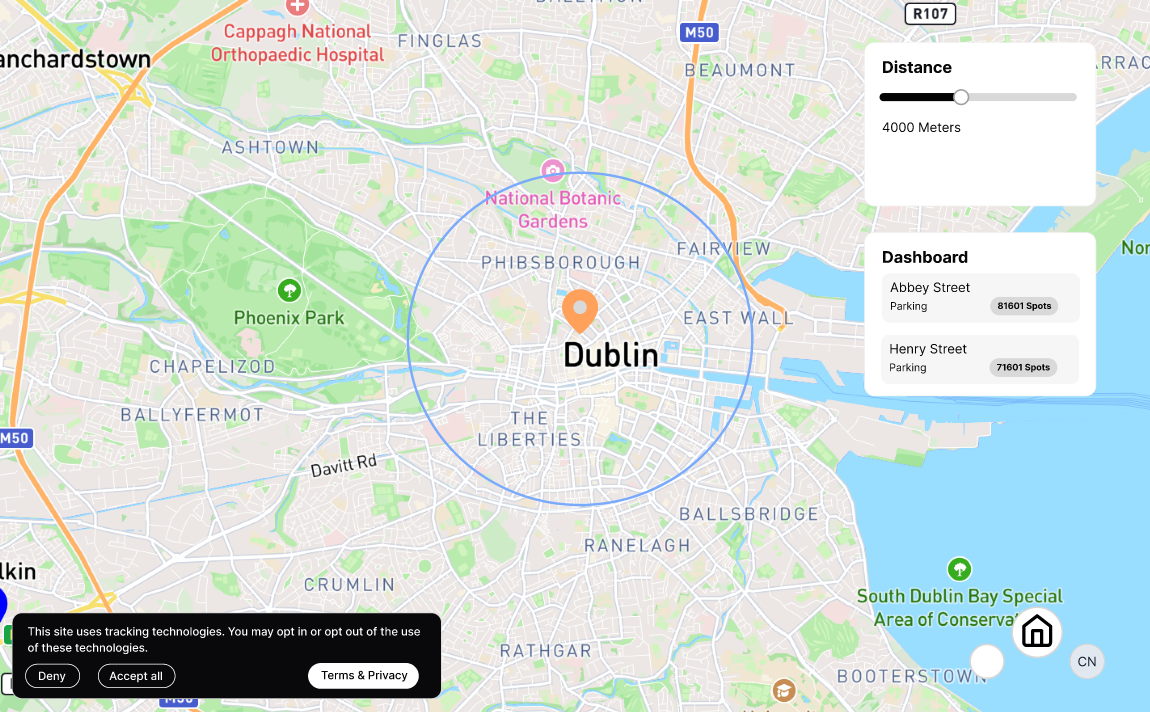
\includegraphics[width=\textwidth]{Figures/fig7.png}}
        \caption{Version 1 of high fidelity prototype}
        \label{fig:plot7}
    \end{minipage}
    \hfill
    \begin{minipage}{0.45\textwidth}
        \centering
        \fbox{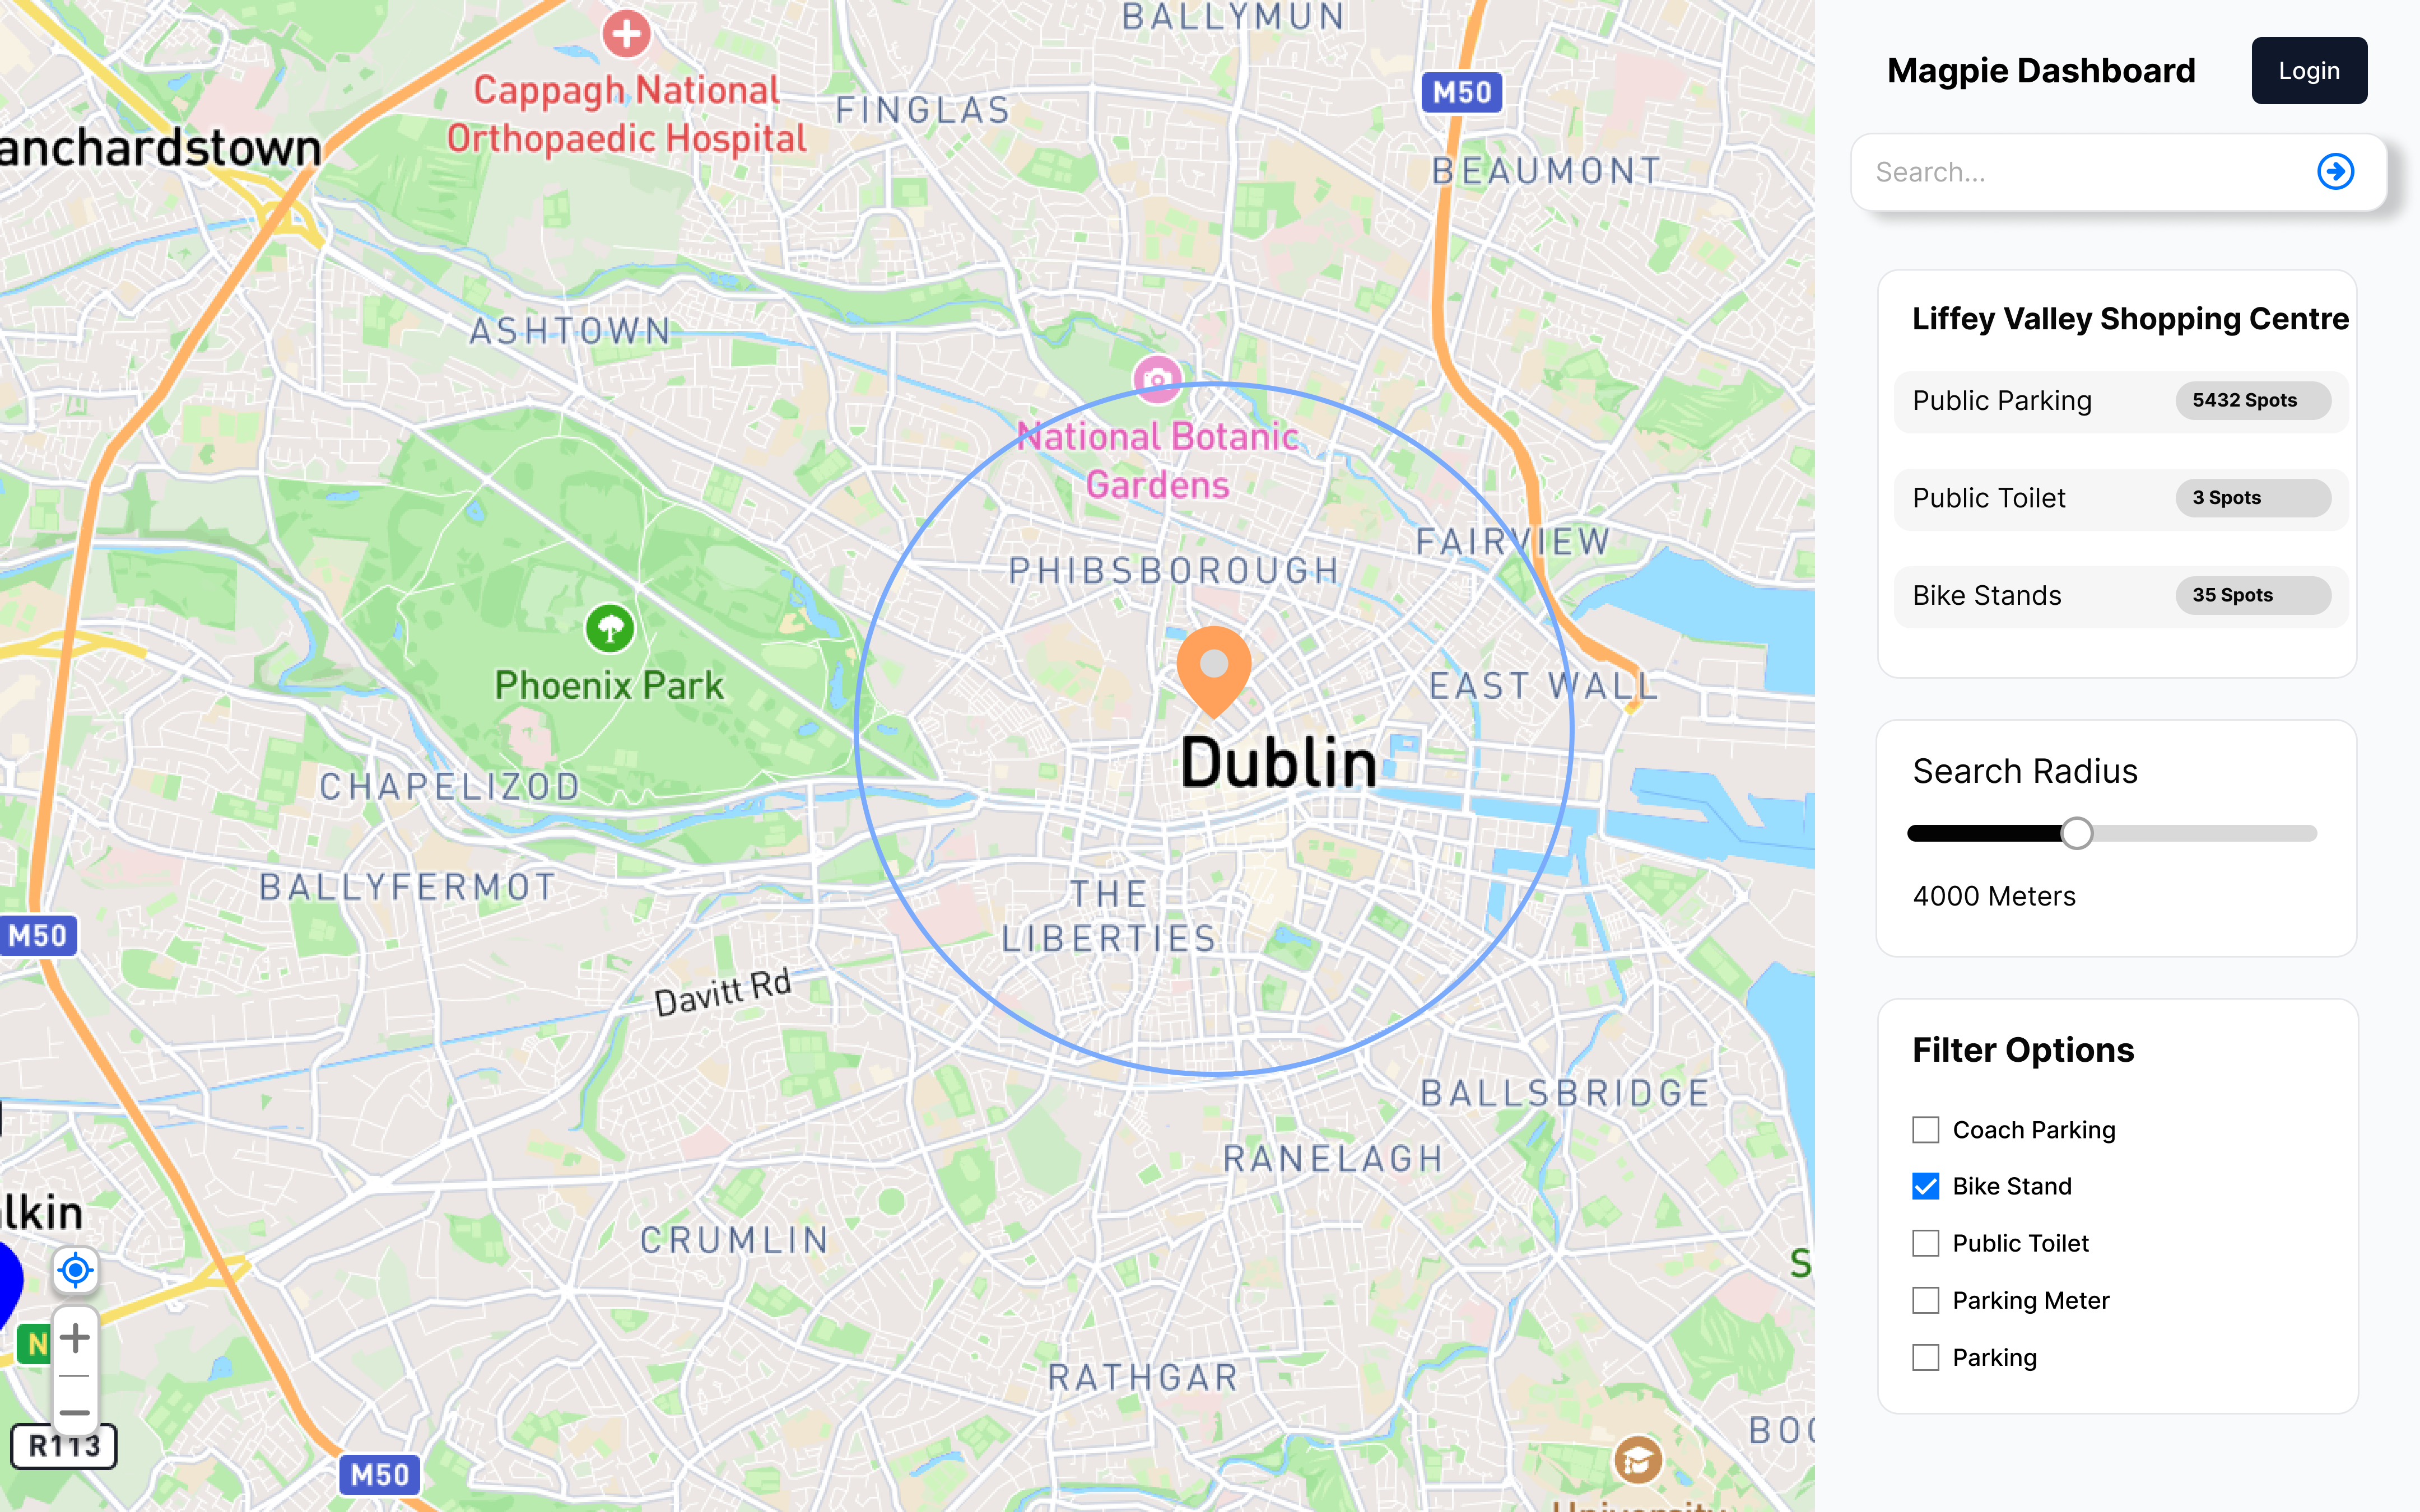
\includegraphics[width=\textwidth]{Figures/fig8.png}}
        \caption{Version 2 of high-fidelity prototype}
        \label{fig:plot8}
    \end{minipage}
\end{figure}

\noindent{}Magpie has remedied the first challenge of fragmented information on
amenities, and through this user evaluation, we hope to address the second challenge
which is making the access to this information easy, quick \& accessible.

\chapter{Experimental Methods}
The goal of the user evaluation is to gain feedback from real users, learn if
Magpie works as expected and assess how user-friendly it is. We will be using 2
main methods to collect both qualitative data through open-ended questions, and
quantitative data from multiple choice questions from which we will derive
insights to improve the Magpie user experience.
\section{Usability Testing}
\subsection{Casual Think-Aloud Protocol}
\begin{enumerate}
    \item \underline{Objective:} Obtain quick feedback on frontend features during the development \& implementation process
    \item \underline{Conditions:} Oral feedback, written notes
    \item \underline{Methodology:}
          \begin{enumerate}
              \item Request feedback from users in the immediate circle
              \item Work together with the user through the app and the feature we want to test
              \item Observe workflow of the user, discuss freely on their manner of interaction with the feature
              \item Build on this feedback to make changes or implement the new feature
          \end{enumerate}
    \item \underline{Baseline \& Evaluation metrics:} No baseline; user experience is evaluated "casually", meaning informally \& subjectively at each person's discretion. This method serves as the "Step 0" of usability testing in helping us implement "Draft 1" of new features.
\end{enumerate}
\subsection{Uncontrolled (Remote)}
\begin{enumerate}
    \item \underline{Objective:} Evaluate user experience in an uncontrolled
          environment, assess overall functioning of Magpie \& identify any
          potential usability issues
    \item \underline{Conditions:} Online followed up by survey
    \item \underline{Methodology:}
          \begin{enumerate}
              \item Share the link to Magpie online to wide user-base to request their participation in testing Magpie
              \item Send them survey to rate their experience
              \item Analyse the responses \& present the results
          \end{enumerate}
    \item \underline{Baseline \& Evaluation metrics:} No baseline; user experience will be evaluated through a 10 question satisfaction survey (figure 2.1) to collect quantitative data only. Minimum number of responses is 20 to produce valuable insights.
\end{enumerate}

\begin{figure}
    \begin{minipage}{\textwidth}
        \centering
        \fbox{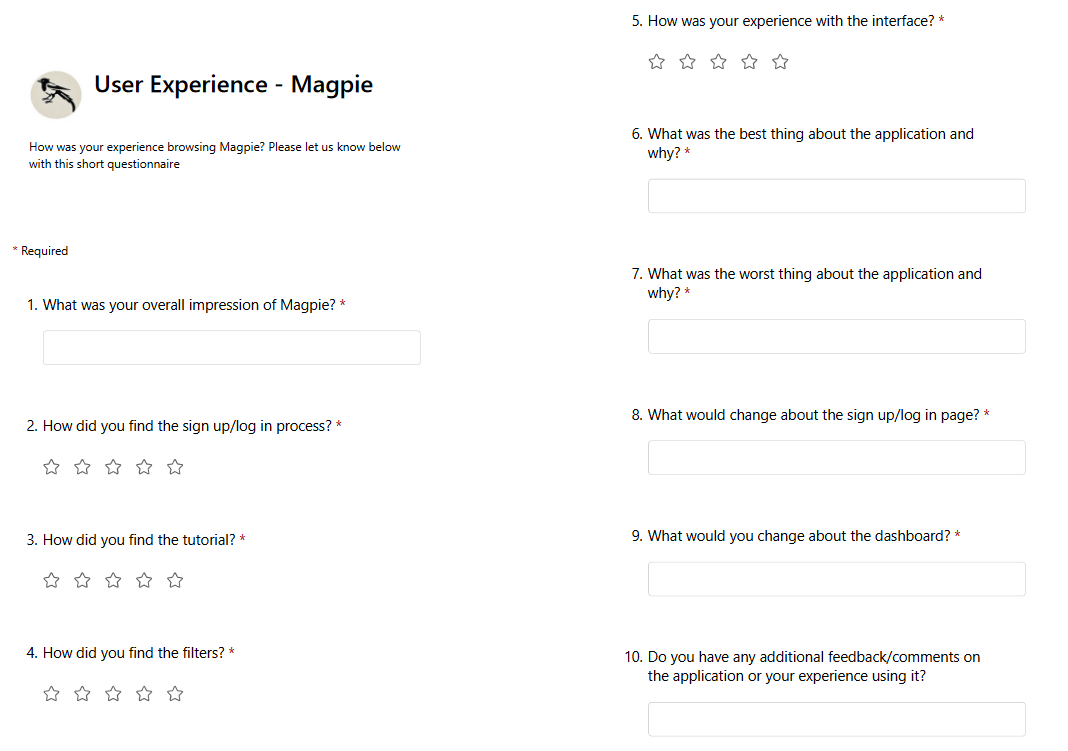
\includegraphics[width=\textwidth]{Figures/fig9.png}}
        \caption{User Experience survey}
        \label{fig:plot9}
    \end{minipage}
\end{figure}

\subsection{Controlled (Remote)}
\begin{enumerate}
    \item \underline{Objective:} Analyze how users interact with Magpie in a
          controlled environment guided by specific instructions and tasks to complete
          \& identify any potential usability issues
    \item \underline{Conditions:} Online through videoconference tools
          (Zoom/GoogleMeet/Teams)
    \item \underline{Methodology:}
          \begin{enumerate}
              \item Reach out to casual users who left their contact email in the market research survey \& request their participation
              \item Schedule the test session
              \item Conduct the test session
              \item Collect qualitative data from users through open-ended questions pre-during-post test
              \item Collect quantitative data from users through user experience survey post-test
              \item Analyse responses \& present results
          \end{enumerate}
    \item \underline{Baseline \& Evaluation metrics:} User experience will be evaluated through a range of metrics shown below in table 2.1  which will measure how the users are working through a series of pre-defined tasks (Table 2.2). These metrics will be measured through observation \& discussion with the users. In addition, quantitative data will be collected through a user experience survey shown in figure 2.1.
\end{enumerate}
\begin{table}[h!]
    \centering
    \caption{Metrics for Controlled Usability testing}
    \label{tab:table1}
    \begin{tabularx}{\textwidth}{|p{0.6\textwidth}|X|X|}
        \hline
        \textbf{Metric}    & \textbf{Threshold}         \\ \hline
        Task Success Rate  & 50\%                       \\ \hline
        Time on Task       & Custom - Dependent on task \\ \hline
        Error Rate         & \hl{look online}           \\ \hline
        Difficulty of task & Custom - Dependent on task \\ \hline
    \end{tabularx}
\end{table}
\begin{table}[h!]
    \centering
    \caption{Tasks for Controlled Usability testing}
    \label{tab:table2}
    \begin{tabularx}{\textwidth}{|p{0.6\textwidth}|X|X|}
        \hline
        \textbf{Task - chronological}                                                                                                                  & \textbf{Completion} & \textbf{Time taken} \\ \hline
        Click on link and load Magpie application                                                                                                      &                     &                     \\ \hline
        Click on Terms and Privacy policy                                                                                                              &                     &                     \\ \hline
        Return to log in page from Terms and Privacy policy page                                                                                       &                     &                     \\ \hline
        Click on "Sign up" and create an account                                                                                                       &                     &                     \\ \hline
        Go through onboarding steps until the end                                                                                                      &                     &                     \\ \hline
        Place cursor on the map in "Phibsborough/Ballyfermot/Temple Bar/Inchicore/Fairview/Dundrum..." area and adjust the radius circle to 250 meters &                     &                     \\ \hline
        Zoom into the area where you placed the cursor until you can clearly see road names on the map                                                 &                     &                     \\ \hline
        Zoom out until you are able to see the radius circle in its entirety                                                                           &                     &                     \\ \hline
        Click on another area of the map "Phibsborough/Ballyfermot/Temple Bar/Inchicore/Fairview/Dundrum..." and increase radius size to 400 meters    &                     &                     \\ \hline
        Choose parking meter amenity in the drop down                                                                                                  &                     &                     \\ \hline
        Remove parking meter amenity from the dropdown                                                                                                 &                     &                     \\ \hline
        Choose Public Toilets and Public Wifi amenities in the drop down                                                                               &                     &                     \\ \hline
        Click on another area of Dublin city "Phibsborough/Ballyfermot/Temple Bar/Inchicore/Fairview/Dundrum..." and reduce radius size to 100 meters  &                     &                     \\ \hline
        \hl{Click on export as png}                                                                                                                    &                     &                     \\ \hline
        Click on the question mark and exit the onboarding at step 3                                                                                   &                     &                     \\ \hline
        Click on avatar and log out                                                                                                                    &                     &                     \\ \hline
    \end{tabularx}
\end{table}
\subsection{Field test (Remote)}
\begin{enumerate}
    \item \underline{Objective:} Analyze how users interact with Magpie in a
          controlled environment guided by their own tasks for their day-to-day work
          \& identify any potential usability issues
    \item \underline{Conditions:} Online through videoconference tools
          (Zoom/GoogleMeet/Teams)
    \item \underline{Methodology:}
          \begin{enumerate}
              \item Reach out to professional users who left their contact
                    email in the market research survey \& request their participation
              \item Schedule the test session
              \item Conduct the test session
              \item Collect qualitative data from users through open-ended questions pre-during-post test
              \item Collect quantitative data through user experience survey post-test
              \item Analyse responses \& present results
          \end{enumerate}
    \item \underline{Baseline \& Evaluation metrics:} No baseline; user
          experience will be evaluated on their feedback through the user experience survey in figure 2.1, complemented by observational analysis.
\end{enumerate}
\section{Expert Review}
We have requested an expert review from a UI/UX professional named Andrea Curley. The goal of this review is to evaluate the user interface of Magpie, rate its user-friendliness in regards to UI/UX general guidelines and the application's compliance with the EAA (European Accessibility Act).\\
The expert review will be conducted online through a videoconference meeting on Teams and will take the following form:
\begin{enumerate}
    \item Presentation of Magpie
    \item Free-roaming of the application by Professor Curley
    \item Questionnaire
    \item Discussion \& end of review
\end{enumerate}
The questionnaire includes questions on visual design, information architecture, data quality \& integration, technical performance, compliance and overall assessment of Magpie as shown in Table 2.3.
\begin{table}[h!]
    \centering
    \caption{Expert Review Questionnaire}
    \label{tab:table3}
    \begin{tabularx}{\textwidth}{|p{0.6\textwidth}|X|X|}
        \hline
        \textbf{Question}                                                                                                                                                                                                                & \textbf{Question type} & \textbf{Answer type} \\ \hline
        How user friendly is the log-in/sign up page?                                                                                                                                                                                    & Closed                 & Multiple choice      \\ \hline
        How user-friendly is the on-boarding process                                                                                                                                                                                     & Closed                 & Multiple choice      \\ \hline
        How effective is the visual hierarchy of the information on the dashboard?                                                                                                                                                       & Closed                 & Multiple choice      \\ \hline
        Rate the clarity of the map visualization                                                                                                                                                                                        & Closed                 & Multiple choice      \\ \hline
        How intuitive is the organization of amenity data categories?                                                                                                                                                                    & Closed                 & Multiple choice      \\ \hline
        Rate the following features from Worst (1) to Best (5) = Onboarding, Radius scaling, filter options completeness, profile menu                                                                                                   & Closed                 & Scale                \\ \hline
        How comprehensive is the amenity data coverage for Dublin city?                                                                                                                                                                  & Closed                 & Multiple choice      \\ \hline
        How valuable do you think this tool would be for the following use cases - 1: Not valuable at all, 5: Extremely valuable = Urban planning, Resource allocation, Planning permissions, Event planning, Education, Travel planning & Closed                 & Scale                \\ \hline
        Any additional comments on why this tool would useful/impractical for the above use cases?                                                                                                                                       & Open-ended             & Text                 \\ \hline
        Evaluate the following technical aspects from Worst (1) to Best (5) = Loading speed, System responsiveness, Data update frequency, Filter functionality, Radius selection                                                        & Closed                 & Scale                \\ \hline
        Rate the application's compliance with the items below from Worst (1) to Best (5) = Accessibility, GIS data standards, GDPR                                                                                                      & Closed                 & Scale                \\ \hline
        Any additional comments regarding our application?                                                                                                                                                                               & Open-ended             & Text
    \end{tabularx}
\end{table}

\chapter{Results}
\section{Usability testing}
\subsection{Casual Think-Aloud Protocol}
\begin{itemize}
    \item Onboarding feature implementation \hl{SAUL}
    \item Dashboard implementation \hl{KAUSTUBH}
    \item Avatar implementation \hl{YUANSHUO}
\end{itemize}
\subsection{Uncontrolled (Remote)}
In Progress
\subsection{Controlled (Remote)}
In Progress
\subsection{Field-test (Remote)}
In Progress

\section{Expert review}
The review provided very valuable insights on Magpie's workflow, user interface and technical components. These were the main takeways:
\begin{itemize}
    \item Andrea was directly taken to the mapview, which was not supposed to happen. After the review, we investigated the cause of this event and uncovered a bug in the authentication
    \item Andrea suggested a landing page introducing Magpie because she felt lost just being taken to the page and nothing happening. Due to the bug explained above, the onboarding did not automatically start.
    \item Regarding onboarding, the user intuitively wants to press on the items being highlighted during the tutorial, which is not possible. That is a current limitation of the way the frontend has been developed.
    \item Still regarding onboarding, Andrea suggested there should be an option to exit the tutorial at any time for users who don't want to sit through it.
    \item Still about onboarding, maybe reduce text but make it more interesting, visually appealing and engaging.
    \item RECOGNITION OVER RECALL
    \item prioritise the items that can be done during this month, and the rest is to be included in the "future work" of the report
    \item currently, its not intuitive where to choose the amenity in the dropdown + icons were not visible enough
    \item zooming into the map!! can we have buttons?
    \item need a connection between the map and the dashboard, especially with the icons, add them to the dashboard
    \item make sure we test magpie on different devices
    \item the hierarchy of items on the dashboard does not make sense, is not intuitive to use. why are all amenities displayed when one is selected and their count displays zero?
    \item looking at the points inside the radius, its currently not obvious what amenity is displaying = the icons are too small and dont stand out enough.
    \item we explained our workflow idea of the design of the dashboard, and when we explained it to her she said "oooh" but it was not obvious and not very intuitive. same for the numbers on the side of each amenity displaying the count. --> we move from bottom up approach (pyramid) instead of the current top down (upside down) approach to the dashboard.
    \item if we want simple clean aesthetic, we need to design the user interface in a way that there is as little room as possible for ambiguity and confusion and guessing games = the user needs to find it easy to move from one feature to another and understand the triggers. currently its looks so slick that the user might not be able to see what they want.
    \item found the parking meter information very useful!
    \item if there are no amenities found in the radius, a message should pop up to tell the user because its not always clear to let the user inspect until their eyes get tired
    \item log out was fine
    \item when trying to log in with credentials that dont exist, a proper error should be returned that "username" doesn't exist, and it should be properly visible
    \item create an account went smoothly
    \item the alert thing for success shouldn't be an alert (my own opinion)
    \item what are the benefits of logging in? we (group) answered that since its a service for professionals, logging in will keep their search, any files they have exported, etc
\end{itemize}


% References & Table of Figures Page
\newpage
\addcontentsline{toc}{chapter}{References}
\chapter*{References}
% Use \bibliography{yourbibfile} with a .bib file if available
\begin{itemize}
    \item Lynn, Theodore et al. (Apr. 2023). “Web Accessibility of Irish Local Government Websites”. In: ICDS 2023 : The
          Seventeenth International Conference on Digital Society.
    \item McGuirk, Pauline M and Andrew MacLaran (2001). “Changing approaches to urban planning in an ‘entrepreneurial
          city’: the case of Dublin”. In: European Planning Studies 9.4, pp. 437–457.
\end{itemize}

\newpage
\addcontentsline{toc}{chapter}{Table of Figures}
\listoffigures
\listoftables

\end{document}
